\documentclass[standalone]{beamer}

\begin{document}
\section{斜率優化}

\begin{frame}{\btitle{形式}}
  \begin{itemize}
    \item 斜率優化又稱凸包優化(convex-hull optimization),幾乎是所有 DP 優化的技巧中,最常見也最容易套用的一種
    \item 常見的 DP 式子形式:$dp(i) = c_i + \max_{j \leq R_i} \{a_jx_i + b_j\}$
    \item 其中 $R_i$ 是一個遞增的序列,而 $c_i$ 是一個與取 max 沒有直接關係的項,可以視為不存在
    \item 通常來說 $a_j$ 或 $b_j$ 會包含 $dp(j)$ 的值,因此在這種情況下會額外的有 $R_i < i$ 的限制
  \end{itemize}
\end{frame}

\begin{frame}{斜率優化}
  \begin{itemize}
    \item 與剛才介紹的單調隊列優化很相似,對於兩個 $j, k$,如果有 $a_k > a_j$ 且 $a_kx + b_k > a_jx + b_j$
    \item 那麼對於所有的 $x^\prime > x$ 而言,$j$ 都不可能是最好的轉移來源
    \item 基於這個觀察,我們可以對已經算好的 $j \leq R_i$,都將 $a_jx + b_j$ 當成是二維平面上的一條直線畫出來
    \item 如此一來,我們的 DP 轉移就變成要查詢 $x_i$ 帶入這些線的最大值,以及要支援動態的將新的直線加入
    \item 先介紹斜率與查詢都是單調的版本,接下來才會進入斜率、查詢不單調的版本
  \end{itemize}
\end{frame}

\begin{frame}{\btitle{斜率、查詢單調}}
  \begin{problem}[ZJ a146 Sliding Window]
    現在你要過 $N$ 個關卡,關卡編號為 $1, 2, \dots, N$,每一個關卡都有一隻怪獸,第 $i$ 個關卡的怪獸的能力值為 $s_i$。在還沒進入任何關卡之前,你有一個初始的技能值 $x$。

    在第 $1, 2, \dots, N - 1$ 關卡中,你可以選擇打倒怪獸,或者是直接逃跑。如果你選擇打倒第 $i$ 隻怪獸,你要花 $f \times s_i$ 的時間打倒怪獸,其中 $f$ 是你當前的技能值。在打倒怪獸後,你的新的能力值會變成 $f_i$。

    你的最終目標是打倒第 $N$ 隻關卡的怪獸,請問在這個過程中,你最少需要花費多少時間。

    \begin{itemize}
      \item $N \leq 2 \times 10^5$
      \item $1 \leq s_1 \leq s_2 \leq \dots \leq s_N \leq 10^6$
      \item $x \geq f_1 \geq f_2 \dots \geq f_N \geq 1$
    \end{itemize}
  \end{problem}
\end{frame}

\begin{frame}{\btitle{斜率、查詢單調}}
  \begin{itemize}
    \item 假設 $f_0 = 0, dp(0) = 0$,應該不難列出以下的 DP 式子:
    \item $dp(i) = \min_{0 \leq j < i}(dp(j) + f_j \times s_i)$
    \item 為了之後講解方便,我們先把所有的 $f_i$ 設成 $-f_i$,我們就可以把 DP 式子轉換成取最大值的形式
    \item $dp(i) = \max_{0 \leq j < i}(dp(j) + f_j \times s_i)$
    \item 並且最後的答案為 $-dp(N)$
  \end{itemize}
\end{frame}

\begin{frame}{\btitle{斜率、查詢單調}}
  \begin{itemize}
    \item $dp(i) = \max_{0 \leq j < i}(dp(j) + f_j \times s_i)$
    \item 如果把上面那個 DP 式寫成斜率優化的形式
    \item 斜率 $a = f_j$,截距 $b = dp(j)$
    \item 轉移 $dp(i)$ 的時候,就是要查詢在 $x = s_i$ 的情況下,那些直線的最大值
    \item 特別的是,我們可以發現:查詢 $s_i$ 跟斜率 $f_j$ 都是\textbf{單調遞增}的
  \end{itemize}
\end{frame}

\begin{frame}{\btitle{斜率、查詢單調}}
  \begin{itemize}
    \item 因此,在這個條件下,這個轉移式會跟前面介紹的單調隊列優化有類似著性質
    \item 如果 $k < j$ 是 $i$ 的最佳轉移來源,那麼對於所有 $i < i^\prime$,從 $j$ 轉移一定會比從 $k$ 轉移來還的好
    \item $a_jx_i + b_j > a_kx_i + b_k \implies a_jx_{i^\prime} + b_j = a_jx_i + a_j(x_{i^\prime} - x_i) + b_j > a_kx_i + a_k(x_{i^\prime} - x_i) + b_k = a_kx_{i^\prime} + b_k$
    \item 有了這個性質以後,我們可以進一步的將時間複雜度壓低
  \end{itemize}
\end{frame}

\begin{frame}{\btitle{斜率、查詢單調}}
  \begin{itemize}
    \item 跟單調隊列一樣,我們維護一個直線的 deque,其中直線由頭至尾斜率遞增
    \item 每次轉移的時候我們可以考慮最前面兩個直線 $L_1, L_2$,比較是否有 $L_1(x_i) < L_2(x_i)$
    \item 根據上面的性質,如果成立的話則代表 $L_1$ 再也不可能成為之後的最佳轉移來源,所以可以將 $L_1$ 移除
    \item 重複這個動作直到現在 deque 最前面的元素 $L$ 還沒有被淘汰,則這時 $L$ 便會是 $i$ 最佳的轉移來源
  \end{itemize}
\end{frame}

\begin{frame}{\btitle{斜率、查詢單調}}
  \begin{itemize}
    \item 解決完查詢以後,接著必須也將加入直線的複雜度降低
    \item 由於斜率單調遞增,我們可以確定現在要加入的直線 $L^\prime$ 一定比現在 deque 中的直線斜率都還要大
    \item 而不難發現,$L^\prime$ 能淘汰的人會是 deque 尾端的一些\textbf{連續}的直線
    \item 假設現在 deque 中最後面的元素為 $L_{-1}$,倒數第二個為 $L_{-2}$
    \item 則可以發現,當 \textbf{$L^\prime$ 與 $L_{-1}$ 的交點比 $L_{-1}$ 以及 $L_{-2}$ 的交點還要左邊}時
    \item $L_{-1}$ 的有效區間會完全的被 $L^\prime$ 覆蓋,再也不可能成為轉移的候選人
  \end{itemize}
\end{frame}


\begin{frame}{\btitle{斜率、查詢單調}}
  \begin{figure}[H]
    \centering
    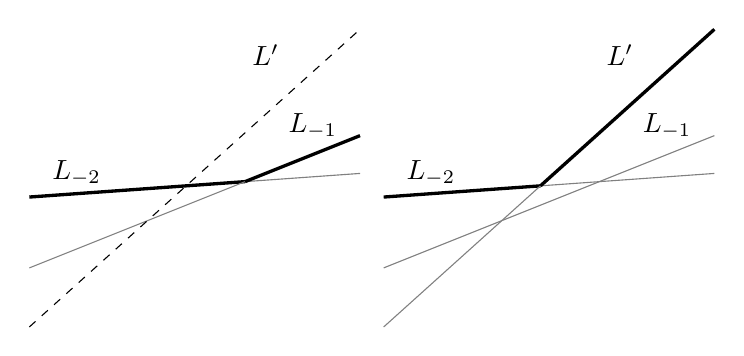
\begin{tikzpicture}[scale=0.3]
      \begin{scope}
      %\draw [domain=0:14,smooth,variable=\x,thick] plot ({\x}, {0.07142857142857142 * \x});
      \draw [domain=0:210/23,smooth,variable=\x,very thick] plot ({\x}, {0.07142857142857142 * \x});
      \draw [domain=210/23:14,smooth,variable=\x,gray] plot ({\x}, {0.07142857142857142 * \x});
      \draw [domain=0:210/23,smooth,variable=\x,gray] plot ({\x}, {0.4 * \x - 3});
      \draw [domain=210/23:14,smooth,variable=\x,very thick] plot ({\x}, {0.4 * \x - 3});
      \draw [domain=0:14,smooth,variable=\x,dashed] plot ({\x}, {0.9 * \x - 5.5});
      \node at (10, 6) (a1) {$L^\prime$};
      \node at (12, 3) (a2) {$L_{-1}$};
      \node at (2, 1) (a3) {$L_{-2}$};
      \end{scope}
      \begin{scope}[shift=({15,0})]
      \draw [domain=0:6.637931,smooth,variable=\x,very thick] plot ({\x}, {0.07142857142857142 * \x});
      \draw [domain=6.637931:14,smooth,variable=\x,gray] plot ({\x}, {0.07142857142857142 * \x});
      \draw [domain=0:14,smooth,variable=\x,gray] plot ({\x}, {0.4 * \x - 3});
      \draw [domain=0:6.637931,smooth,variable=\x,gray] plot ({\x}, {0.9 * \x - 5.5});
      \draw [domain=6.637931:14,smooth,variable=\x,very thick] plot ({\x}, {0.9 * \x - 5.5});
      \node at (10, 6) (a1) {$L^\prime$};
      \node at (12, 3) (a2) {$L_{-1}$};
      \node at (2, 1) (a3) {$L_{-2}$};
      \end{scope}
    \end{tikzpicture}
    \caption{$L^\prime$ 與 $L_{-2}$ 合力將 $L_{-1}$ 淘汰}
  \end{figure}
\end{frame}


\begin{frame}{\btitle{斜率、查詢單調}}
  \begin{itemize}
    \item 至此,單調版本的斜率優化已經成形
    \item 而根據與單調隊列優化相似的論述,每條直線只會被加入一次,並至多被移除一次
    \item 由於使用 deque,每次加入以及刪除都是 $O(1)$,所以總時間複雜度可以降為 $O(N)$
    \item 至於將最大值改為最小值的版本,則留給讀者自行推導
  \end{itemize}
\end{frame}

\begin{frame}[fragile]{\btitle{斜率、查詢單調}}
  \begin{minted}[breaklines]{cpp}
    typedef long long ll;

    struct Line {
      ll a, b; // 一條 ax + b 的直線
      Line(ll _a, ll _b): a(_a), b(_b){}
      ll operator()(const ll x) {
        return a * x + b;
      }
    };
  \end{minted}
\end{frame}

\begin{frame}[fragile]{\btitle{斜率、查詢單調}}
  \begin{minted}[breaklines]{cpp}
    bool check(Line l1, Line l2, Line l3) {
      // l1 是講義中的 L_{-2},l2 是講義中的 L_{-1},l3 是想要新增的直線
      // double v12 = (l1.b - l2.b) / (l2.a - l1.a) 
      // double v23 = (l2.b - l3.b) / (l3.a - l2.a)
      // return v12 >= v13
      // 但是上面的方法會有浮點數誤差,因此在這裡只考慮使用整數運算,方法如下:
      return (l3.a - l2.a) * (l1.b - l2.b) >= (l3.b - l2.b) * (l1.a - l2.a);
    }
  \end{minted}
\end{frame}

\begin{frame}[fragile]{\btitle{斜率、查詢單調}}
  \begin{minted}[breaklines]{cpp}
    void solve(int n) {
      for (int i = 1; i <= n; ++i) {
        while ((int)dq.size() >= 2 && dq[0](s[i]) <= dq[1](s[i])) {
          // 把比較差的線丟掉,注意到這邊寫 <= 或 < 其實都 ok
          dq.pop_front();
        }
        dp[i] = dq[0](s[i]);
        Line l = Line(f[i], dp[i]);
        while ((int)dq.size() >= 2 && check(dq[(int)dq.size() - 2], dq[(int)dq.size() - 1], l)) {
          // 把新的線加進去,看看 L_{-2} 跟 L 有沒有辦法把 L_{-1} 殺掉
          dq.pop_back();
        }
        dq.push_back(l);
      }
    }
  \end{minted}
\end{frame}

\begin{frame}{\btitle{會單調過期的斜率、查詢單調}}
  \begin{itemize}
    \item 有時候在斜率單調的優化時,會遇到一條線再加入之後會單調過期(也就是過期的時間與斜率都具有單調性)的版本
    \item 一個例子就是當 DP 轉移只能轉移前 $K$ 項時,那 $dp(i)$ 所代表的那條線在 $i + K$ 的時候就會被迫移出凸包
    \item 直接來看例題吧~
  \end{itemize}
\end{frame}

\begin{frame}{\btitle{會單調過期的斜率、查詢單調}}
  \begin{problem}[NEOJ 186 烏龜疊疊樂改]
    給你一個長度為 $N$ 的序列 $a_1, a_2, \dots, a_N$,以及一個常數 $K$。

    請你把序列分成 $M$ 段,每段的長度不超過 $K$。假設第 $i$ 段的開頭為 $l_i$,結尾為 $r_i$。請你最大化:

    $\sum_{i = 1}^{M}((\sum_{x = l_i}^{r_i}a_x) \times i - (r_i - l_i + 1)^2)$

    % $(1 \leq K \leq N \leq 5 \times 10^5)$
    \begin{itemize}
      \item $1 \leq K \leq N \leq 5 \times 10^5$
    \end{itemize}

    註:上面的式子跟原題稍微不太一樣
  \end{problem}
\end{frame}

\begin{frame}{\btitle{會單調過期的斜率、查詢單調}}
  \begin{itemize}
    \item 把 $a$ 序列進行翻轉(reverse),並且定義 $pre$ 陣列為 $a$ 序列的前綴和陣列: $pre_i = \sum_{x = 1}^{i} a_x$
    \item 定義 $dp(i)$ 代表我們看到序列的第 $i$ 項時,可能的最大值
    \item 則我們可以列出以下的 DP 式子
    \item $dp(i) = pre_i + \max_{\max(i - K, 0) \leq j < i}(dp(j) - (i - j)^2)$
    \item 把式子改寫成斜率優化的形式(斜率為 $2j$,截距為 $dp(j) - j^2$)
    \item $dp(i) = pre_i - i^2 + \max_{\max(i - K, 0) \leq j < i}(2j \times i + dp(j) - j^2)$
    \item 而我們可以注意到,因為每段的長度不能超過 $K$,因此\textbf{轉移的線會單調過期}
  \end{itemize}
\end{frame}

\begin{frame}{\btitle{會單調過期的斜率、查詢單調}}
  \begin{itemize}
    \item 考慮新的直線加入凸包時的狀況
    \item 當新的直線 $L$ 與凸包中倒數第二的直線 $L_{-2}$ 合力「殺掉」凸包中最後的直線 $L_{-1}$ 時
    \item 若直線會被淘汰掉,那麼其實不能直接將 $L_{-1}$ 移除,因為 $L_{-1}$ 能存活的時間比 $L_{-2}$ 久
    \item 當 $L_{-2}$ 過期之後,$L_{-1}$ 可能重新「復活」變成最佳轉移來源
  \end{itemize}
\end{frame}

\begin{frame}{\btitle{會單調過期的斜率、查詢單調}}
  \begin{figure}[H]
    \centering
    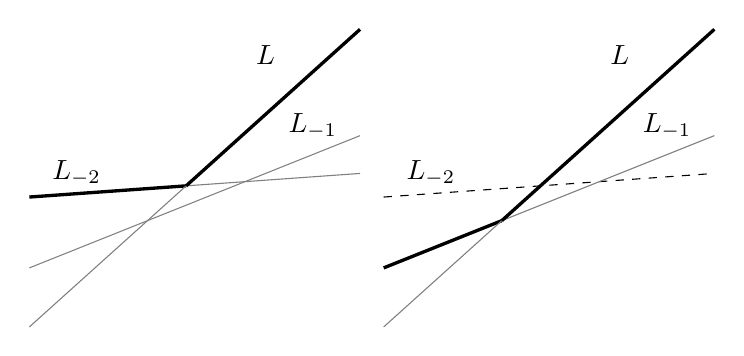
\begin{tikzpicture}[scale=0.3]
      \begin{scope}
      %\draw [domain=0:14,smooth,variable=\x,thick] plot ({\x}, {0.07142857142857142 * \x});
      \draw [domain=0:6.637931,smooth,variable=\x,very thick] plot ({\x}, {0.07142857142857142 * \x});
      \draw [domain=6.637931:14,smooth,variable=\x,gray] plot ({\x}, {0.07142857142857142 * \x});
      \draw [domain=0:14,smooth,variable=\x,gray] plot ({\x}, {0.4 * \x - 3});
      \draw [domain=0:6.637931,smooth,variable=\x,gray] plot ({\x}, {0.9 * \x - 5.5});
      \draw [domain=6.637931:14,smooth,variable=\x,very thick] plot ({\x}, {0.9 * \x - 5.5});
      \node at (10, 6) (a1) {$L$};
      \node at (12, 3) (a2) {$L_{-1}$};
      \node at (2, 1) (a3) {$L_{-2}$};
      \end{scope}
      \begin{scope}[shift=({15,0})]
      \draw [domain=0:14,smooth,variable=\x,dashed] plot ({\x}, {0.07142857142857142 * \x});
      \draw [domain=0:5,smooth,variable=\x,very thick] plot ({\x}, {0.4 * \x - 3});
      \draw [domain=5:14,smooth,variable=\x,gray] plot ({\x}, {0.4 * \x - 3});
      \draw [domain=0:5,smooth,variable=\x,gray] plot ({\x}, {0.9 * \x - 5.5});
      \draw [domain=5:14,smooth,variable=\x,very thick] plot ({\x}, {0.9 * \x - 5.5});
      \node at (10, 6) (a1) {$L$};
      \node at (12, 3) (a2) {$L_{-1}$};
      \node at (2, 1) (a3) {$L_{-2}$};
      \end{scope}
    \end{tikzpicture}
    \caption{當 $L_{-2}$ 過期之後,$L_{-1}$ 又重回凸包上。}
  \end{figure}
\end{frame}

\begin{frame}{\btitle{會單調過期的斜率、查詢單調}}
  \begin{itemize}
    \item 那這個時候 $L$ 與 $L_{-2}$ 合力殺掉 $L_{-1}$ 的條件就是「就算 $L_{-2}$ 過期 $L$ 還是一直比 $L_{-1}$ 優」
    \item 也就是說在檢查交點的時候,除了判斷 $(L, L_{-1})$ 與 $(L_{-2}, L_{-1})$ 這兩組交點外,還需要考慮 $L_{-2}$ 過期時的查詢位置 $x$
    \item 所以\textbf{只要當 $(L, L_{-1})$ 的交點比 $x$ 還有 $(L_{-2}, L_{-1})$ 都還要左邊時,才能完全淘汰 $L_{-1}$}。
  \end{itemize}
\end{frame}



\begin{frame}[fragile]{\btitle{會單調過期的斜率、查詢單調}}
  \begin{minted}[breaklines]{cpp}
    ll DivCeil(ll x, ll y) { // 計算 x / y 取上高斯,不管 x, y 的正負情況都適用
      return x / y + (((x < 0) != (y > 0)) && (x % y));
    }

    bool check(Line l1, Line l2, Line l3) {
      // 注意到這題點只有定義在整數上,因此可以用下面的技巧來避免浮點數
      ll v1 = DivCeil((l1.b - l2.b), (l2.a - l1.a)); // L_{-2} 與 L_{-1} 的交點。在這邊代表 L_{-1} 第一個超越 L_{-2} 的整數點
      ll v2 = DivCeil((l2.b - l3.b), (l3.a - l2.a)); // L_{-1} 與 L 的交點。在這邊代表 L 第一個超越 L_{-1} 的整數點
      ll v3 = l1.i + k; // L_{-2} 最後一個合法的位置, v3 + 1 就過期了
      return v2 <= v3 && v2 <= v1;
    }
  \end{minted}
\end{frame}

\begin{frame}{斜率優化}
  \begin{itemize}
    \item 從這邊開始,要介紹斜率優化最 general 的版本
    \item 同樣的,我們先假設 DP 式子是以下的形式:
    \item $dp(i) = c_i + \max_{j \leq R_i} \{a_jx_i + b_j\}$
    \item 跟前面的章節類似,我們會把 $a_jx + b_j$ 當成二維平面上的一條直接去畫出來
    \item 讓 DP 轉移變成帶入查詢 $x_i$ 得到最大值,並且我們要支援新的直線的加入
  \end{itemize}
\end{frame}

\begin{frame}{斜率優化}
  \begin{itemize}
    \item 由於最大值一定在這些直線所形成的下凸包中(若為最小值的話改為上凸包)
    \item 我們可以將所有的線照斜率排好,並且對於每條直線維護它出現在凸包上的 $x$ 軸範圍
    \item 實作上可以直線 $L$ 維護 $p_L$,代表 $L$ 最左從 $p_L$ 開始出現在凸包上( $L$ 右界就是下一條線的左界)
    \item 如此一來,每次查詢 $x$ 的時候只要二分搜到斜率最大的 $L^\prime$,使得 $p_L^\prime \leq x$ 即可。
  \end{itemize}
\end{frame}

\begin{frame}{斜率優化}
  \begin{figure}[H]
  \centering
  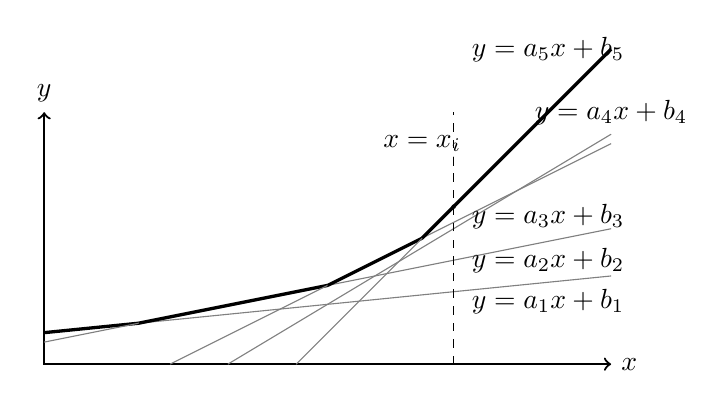
\begin{tikzpicture}[scale=0.4]
      % Draw axes
      \draw [<->,thick] (0,8) node (yaxis) [above] {$y$}
          |- (18,0) node (xaxis) [right] {$x$};

      \draw [domain=0:3,smooth,variable=\x,very thick] plot ({\x}, {0.1 * \x + 1});
      \draw [domain=3:18,smooth,variable=\x,gray] plot ({\x}, {0.1 * \x + 1});
      \draw [domain=0:3,smooth,variable=\x,gray] plot ({\x}, {0.2 * \x + 0.7});
      \draw [domain=3:9,smooth,variable=\x,very thick] plot ({\x}, {0.2 * \x + 0.7});
      \draw [domain=9:18,smooth,variable=\x,gray] plot ({\x}, {0.2 * \x + 0.7});
      \draw [domain=4:9,smooth,variable=\x,gray] plot ({\x}, {0.5 * \x - 2});
      \draw [domain=9:12,smooth,variable=\x,very thick] plot ({\x}, {0.5 * \x - 2});
      \draw [domain=12:18,smooth,variable=\x,gray] plot ({\x}, {0.5 * \x - 2});
      \draw [domain=5.8333:18,smooth,variable=\x,gray] plot ({\x}, {0.6 * \x - 3.5});
      \draw [domain=8:12,smooth,variable=\x,gray] plot ({\x}, {\x - 8});
      \draw [domain=12:18,smooth,variable=\x,very thick] plot ({\x}, {\x - 8});
      \coordinate (x) at (13, 5);
      \draw [domain=0:8,smooth,variable=\y,dashed] plot ({13}, {\y});
      \node at (16, 2) (a1) {$y = a_1x + b_1$};
      \node at (16, 3.3) (a2) {$y = a_2x + b_2$};
      \node at (16, 4.7) (a3) {$y = a_3x + b_3$};
      \node at (18, 8) (a4) {$y = a_4x + b_4$};
      \node at (16, 10) (a5) {$y = a_5x + b_5$};
      \node at (12, 7) (x13) {$x = x_i$};
      \fill (x) circle (2pt);
  \end{tikzpicture}
  \caption{將所有 $j \leq R_i$ 的 $y = a_jx + b_j$ 都畫在二維平面上。其中 $y = a_4x + b_4$ 並不在凸包上,不可能成為轉移來源。$x = x_i$ 的最佳轉移來源為 $y = a_5x + b_5$。}
  \end{figure}
\end{frame}

\begin{frame}{斜率優化}
  \begin{itemize}
    \item 解決了查詢之後,接著必須考慮當 $R_i$ 增加的時候,該怎麼維護這個凸包
    \item 首先,可以用斜率來二分搜以找到新加入的直線在凸包上的位置
    \item 加入了之後,有一些原本在凸包上的直線會從凸包中被移除,有一些的有效區間則會被修改,且這些被淘汰的直線原本在凸包會是一個\textbf{連續的區間}
    \item 具體來說,假設現在凸包中的直線斜率由小至大分別為 $(L_1, L_2, \ldots, L_k)$,且新的直線 $L^\prime$ 被加入凸包的位置為 $L_{i}$ 以及 $L_{i + 1}$ 之間,則會存在 $j$ 與 $k$ 使得 $\{L_k, L_{k + 1} \ldots, L_{i}, L_{i + 1}, \ldots, L_{j} \}$ 被 $L^\prime$ 淘汰,且 $L_{k - 1}$ 與 $L_{j + 1}$ 的有效區間被更新
  \end{itemize}
\end{frame}

\begin{frame}{斜率優化}
  \begin{itemize}
    \item 那要如何更新有效區間呢?
    \item 由於 $L^\prime$ 不能完全淘汰 $L_{j + 1}$ 的原因便是 $L^\prime$ 在完全打敗 $L_{j + 1}$ 之前就與 $L_{j + 1}$ 相交了
    \item 因為 $L^\prime$ 的斜率小於 $L_{j + 1}$,相交就代表在交點 $x_0$ 之後,$L^\prime(x)$ 的值就不可能在比 $L_{j + 1}(x)$ 來得大了
    \item 所以 $L^\prime$ 的有效區間的右界就到 $x_0$,而 $L_{j + 1}$ 的有效左界則會被改為 $x_0$
    \item 同樣的論述可以套用在 $L_{k - 1}$ 上,不過由於 $L_{k - 1}$ 的斜率小於 $L^\prime$,會變成改動 $L_{k - 1}$ 的有效右界
  \end{itemize}
\end{frame}

\begin{frame}{斜率優化}
\begin{figure}[H]
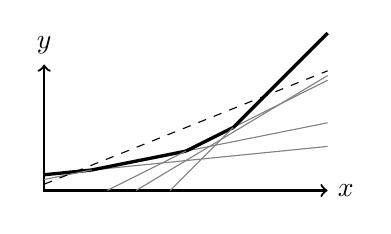
\begin{tikzpicture}[scale=0.2]
    % Draw axes
    \draw [<->,thick] (0,8) node (yaxis) [above] {$y$}
        |- (18,0) node (xaxis) [right] {$x$};

    \draw [domain=0:3,smooth,variable=\x,very thick] plot ({\x}, {0.1 * \x + 1});
    \draw [domain=3:18,smooth,variable=\x,gray] plot ({\x}, {0.1 * \x + 1});
    \draw [domain=0:3,smooth,variable=\x,gray] plot ({\x}, {0.2 * \x + 0.7});
    \draw [domain=3:9,smooth,variable=\x,very thick] plot ({\x}, {0.2 * \x + 0.7});
    \draw [domain=9:18,smooth,variable=\x,gray] plot ({\x}, {0.2 * \x + 0.7});
    \draw [domain=4:9,smooth,variable=\x,gray] plot ({\x}, {0.5 * \x - 2});
    \draw [domain=9:12,smooth,variable=\x,very thick] plot ({\x}, {0.5 * \x - 2});
    \draw [domain=12:18,smooth,variable=\x,gray] plot ({\x}, {0.5 * \x - 2});
    \draw [domain=5.8333:18,smooth,variable=\x,gray] plot ({\x}, {0.6 * \x - 3.5});
    \draw [domain=8:12,smooth,variable=\x,gray] plot ({\x}, {\x - 8});
    \draw [domain=12:18,smooth,variable=\x,very thick] plot ({\x}, {\x - 8});
    %\draw [domain=0:2,smooth,variable=\x,thick] plot ({\x}, {0.4 * \x + 0.4});
    \draw [domain=0:18,smooth,variable=\x,dashed] plot ({\x}, {0.4 * \x + 0.4});
    %\draw [domain=14:18,smooth,variable=\x,thick] plot ({\x}, {0.4 * \x + 0.4});
\end{tikzpicture}
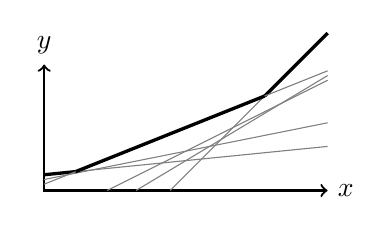
\begin{tikzpicture}[scale=0.2]
    % Draw axes
    \draw [<->,thick] (0,8) node (yaxis) [above] {$y$}
        |- (18,0) node (xaxis) [right] {$x$};

    \draw [domain=0:2,smooth,variable=\x,very thick] plot ({\x}, {0.1 * \x + 1});
    \draw [domain=2:18,smooth,variable=\x,gray] plot ({\x}, {0.1 * \x + 1});
    \draw [domain=0:3,smooth,variable=\x,gray] plot ({\x}, {0.2 * \x + 0.7});
    \draw [domain=3:9,smooth,variable=\x,gray] plot ({\x}, {0.2 * \x + 0.7});
    \draw [domain=9:18,smooth,variable=\x,gray] plot ({\x}, {0.2 * \x + 0.7});
    \draw [domain=4:9,smooth,variable=\x,gray] plot ({\x}, {0.5 * \x - 2});
    \draw [domain=9:12,smooth,variable=\x,gray] plot ({\x}, {0.5 * \x - 2});
    \draw [domain=12:18,smooth,variable=\x,gray] plot ({\x}, {0.5 * \x - 2});
    \draw [domain=5.8333:18,smooth,variable=\x,gray] plot ({\x}, {0.6 * \x - 3.5});
    \draw [domain=8:14,smooth,variable=\x,gray] plot ({\x}, {\x - 8});
    \draw [domain=14:18,smooth,variable=\x,very thick] plot ({\x}, {\x - 8});
    \draw [domain=0:2,smooth,variable=\x,gray] plot ({\x}, {0.4 * \x + 0.4});
    \draw [domain=2:14,smooth,variable=\x,very thick] plot ({\x}, {0.4 * \x + 0.4});
    \draw [domain=14:18,smooth,variable=\x,gray] plot ({\x}, {0.4 * \x + 0.4});
\end{tikzpicture}
\caption{加入新的直線後,$y = a_2x + b_2$ 以及 $y = a_3x + b_3$ 被完全淘汰。$y = a_1x + b_1$ 與 $y = a_5x + b_5$ 的有效右界以及有效左界分別被改為其與新線的交點。}
\end{figure}
\end{frame}

\begin{frame}{斜率優化}
  \begin{itemize}
    \item 那這樣的時間複雜度會是多少呢?
    \item 每次查詢以及插入需要使用若干次二分搜,一次為 $O(\log{N})$
    \item 並且在插入後會刪掉一些數量不等的元素,一次刪除的複雜度也是 $O(\log{N})$
    \item 這邊我們可以套用在上一個章節所使用的\textbf{均攤分析}來計算:每一條直線只會被加入凸包中一次,且至多只會被移除一次
    \item 每次加入跟移除都是 $O(\log{N})$,所以均攤下來每一次操作都是 $O(\log{N})$ 的
    \item 如此一來,我們便得到一個時間複雜度 $O(\log{N})$ 的算法,相比原本的 $O(N^2)$ 是一個極大的改進
  \end{itemize}
\end{frame}

\begin{frame}{斜率優化}
  \begin{itemize}
    \item 實作上,由於我們需要支援:
    \item 對於給定的 $x$,二分搜斜率最大的 $L$ 使得 $p_L \leq x$
    \item 對於一條直線 $L$,二分搜找到它在凸包的位置並且插入
    \item 刪除一條直線
  \end{itemize}
\end{frame}

\begin{frame}{斜率優化}
  \begin{itemize}
    \item 一個理想的結構為一個平衡二元樹
    \item 由於實作方便,通常都是使用 \texttt{std::set} 配合自定義的直線 \texttt{Line}
    \item 不過在我們要支援的操作中,有兩種二分搜的基準(斜率、有效區間),直接套用 \texttt{std::set} 的話可能會有一些小問題
    \item 一個直覺的處理方法是維護兩個 \texttt{std::set},不過這樣不僅會讓 code 量變很大而且還會讓常數變大,並不是一個實惠的做法。以下介紹兩種處理的方法,讀者可以自行參考使用
    \begin{enumerate}
      \item 使用一個全域的變數 \texttt{flag} 來記錄現在要使用哪一種二分搜的基準,並且在 \texttt{Line} 的比較運算子中根據 \texttt{flag} 的值來調整內容
      \item 重載 \texttt{Line} 的比較運算子:一個與 \texttt{Line} 比較(斜率)、一個與整數比較(有效區間)
    \end{enumerate}
    \item 範例程式碼使用第二種方法,並且直接繼承 \texttt{std::multiset} 以減少實作負擔
    \item 值得注意的是,在大部分的問題中查詢都是整數,因此有效區間以及交點的計算都可以在整數上計算以減少浮點數誤差
  \end{itemize}
\end{frame}

\begin{frame}{\btitle{例題}}
  \begin{problem}[CSES 2085 Monster Game II]
    現在你要過 $N$ 個關卡,關卡編號為 $1, 2, \dots, N$,每一個關卡都有一隻怪獸,第 $i$ 個關卡的怪獸的能力值為 $s_i$。在還沒進入任何關卡之前,你有一個初始的技能值 $x$。

    在第 $1, 2, \dots, N - 1$ 關卡中,你可以選擇打倒怪獸,或者是直接逃跑。如果你選擇打倒第 $i$ 隻怪獸,你要花 $f \times s_i$ 的時間打倒怪獸,其中 $f$ 是你當前的技能值。在打倒怪獸後,你的新的能力值會變成 $f_i$。

    你的最終目標是打倒第 $N$ 隻關卡的怪獸,請問在這個過程中,你最少需要花費多少時間。

    % $(N \leq 2 \times 10^5)$
    \begin{itemize}
      \item $N \leq 2 \times 10^5$
    \end{itemize}
  \end{problem}
\end{frame}

\begin{frame}{斜率優化}
  \begin{itemize}
    \item 假設 $f_0 = 0, dp(0) = 0$,應該不難列出以下的 DP 式子:
    \item $dp(i) = \min_{0 \leq j < i}(dp(j) + f_j \times s_i)$
    \item 為了之後講解方便,我們先把所有的 $f_i$ 設成 $-f_i$,我們就可以把 DP 式子轉換成取最大值的形式:
    \item $dp(i) = \max_{0 \leq j < i}(dp(j) + f_j \times s_i)$
    \item 並且最後的答案為 $-dp(N)$
    \item 而跟前面那個例題不同是,這邊的斜率、查詢不再是單調的。因此,就需要使用上面那個技巧
  \end{itemize}
\end{frame}

\begin{frame}{\btitle{用 CDQ 解斜率非單調的斜率優化}}
  \begin{itemize}
    \item 在上個小章節,我們成功用 $O(N \log N)$ 的時間內,解決了斜率非單調的斜率優化
    \item 不過,動態凸包其實沒有想像中那麼好寫
    \item 但是,相對來說,如果斜率、詢問都是單調的話,世界會變得非常的美好,實作的難易度也會下降很多
    \item 我們有沒有辦法把非單調的東西變成單調呢?
    \item 答案是肯定的
  \end{itemize}
\end{frame}

\begin{frame}{\btitle{用 CDQ 解斜率非單調的斜率優化}}
  \begin{itemize}
    \item 考慮以下分治法:
    \item 如果 $L == R$,結束遞迴
    \item 否則,依序執行以下步驟:
    \begin{itemize}
      \item 遞迴計算左半部 $[L, mid]$ 的 DP 值。
      \item 用左半部 $[L, mid]$ 算出來的 DP 值,更新右半部 $[mid + 1, R]$ 的 DP 值。
      \item 遞迴計算右半部 $[mid + 1, R]$ 的 DP 值。
    \end{itemize}
  \end{itemize}
\end{frame}

\begin{frame}{\btitle{用 CDQ 解斜率非單調的斜率優化}}
  \begin{itemize}
    \item 應該不難發現,每個 DP 值在計算的過程中,\textbf{都會被所有可能的轉移點嘗試轉移}
    \item 因此,上述演算法的正確性是可以保證的
    \item 但是,時間複雜度呢?
    \item 如果左半部 DP 值更新右半部的部份,我們單純使用 $O(N^2)$ 轉移,會讓複雜度變成 $T(N) = 2T(\frac{N}{2}) + O(N^2)$,會使得最後的複雜度為 $O(N^2)$
    \item 但,「用左半部更新右半部」這個部份,\textbf{其實就是個斜率單調、詢問單調的問題}
  \end{itemize}
\end{frame}

\begin{frame}{\btitle{用 CDQ 解斜率非單調的斜率優化}}
  \begin{itemize}
    \item 因為我們\textbf{可以把左半部的線按照斜率排序}、\textbf{把右半部的詢問按照詢問大小排序}
    \item 可以這麼做的理由是因為,我們已經知道所有左半邊的 DP 值(也就是說,我們已經知道所有的線),同時我們也可以知道所有右半部的詢問
    \item 因此,我們就可以\textbf{自由的決定他們的順序},得到一個好的順序之後,我們就可以好好的方便做事了!
    \item 也因此,「用左半部更新右半部」這個部份,我們可以花 $O(N \log N)$ 的時間排序,並且花 $O(N)$ 的時間內解決。因此,整體複雜度就變成 $T(N) = 2T(\frac{N}{2} + O(N \log N))$,得到 $T(N) = O(N \log^2 N)$ 的複雜度
    \item 可以參考講義上面的範例程式碼~
  \end{itemize}
\end{frame}


\end{document}
